\chapter{Planificación y costes}

Definir claramente de acuerdo con el tutor los “paquetes de trabajo” (PTs), identificando claramente los entregables resultantes de cada uno de ellos. Esto definirá claramente los resultados del proyecto. Pueden usarse Diagramas de Gantt o cualquier herramienta o metodología siempre que facilite la visualización secuencial y dependencias entre los PT. En este mismo capítulo se incluir un presupuesto –ajustado en lo posible a la realidad- que incluya recursos humanos y materiales, así como cualquier dato que determine la viabilidad del proyecto.


%\begin{figure}[h]
%	\centering
%	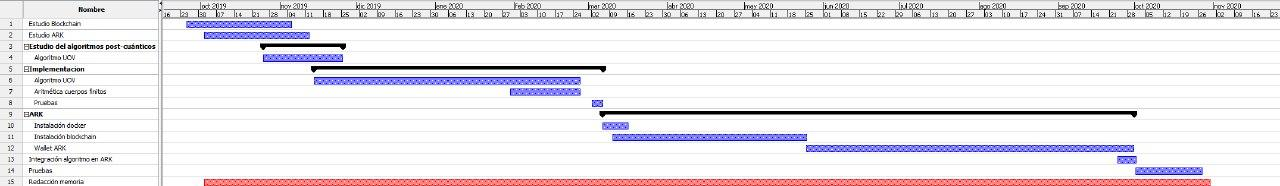
\includegraphics[width=1.5\textwidth]{figuras/Gantt.jpg}
%	\caption{Comparativa de la capacidad de cómputo de un ordenador clásico con un ordenador cuántico\cite{clasica-vs-cuantica}}
%	\label{fig:comp-clasica-cuantica}
%\end{figure}


\begin{figure}[h]
	\centering
	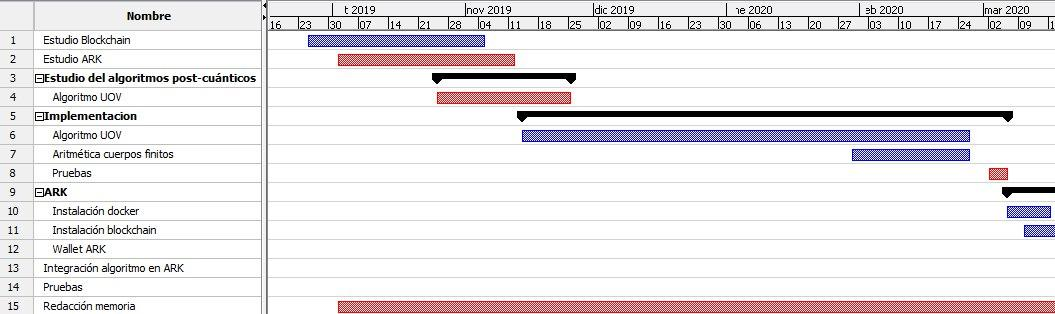
\includegraphics[width=16cm,height=6.5cm]{figuras/Gantt_1.jpg}
	\caption{Comparativa de la capacidad de cómputo de un ordenador clásico con un ordenador cuántico\cite{clasica-vs-cuantica}}
	\label{fig:comp-clasica-cuantica}
\end{figure}

\begin{figure}[h]
	\centering
	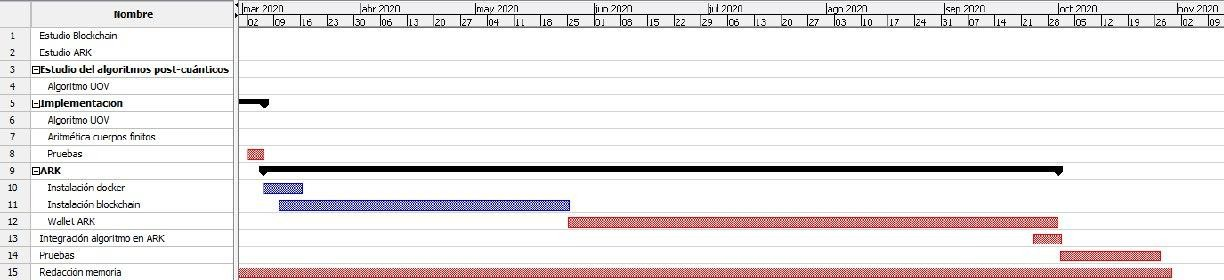
\includegraphics[width=15cm,height=6.5cm]{figuras/Gantt_2.jpg}
	\caption{Comparativa de la capacidad de cómputo de un ordenador clásico con un ordenador cuántico\cite{clasica-vs-cuantica}}
	\label{fig:comp-clasica-cuantica}
\end{figure}

\begin{figure}[h]
	\centering
	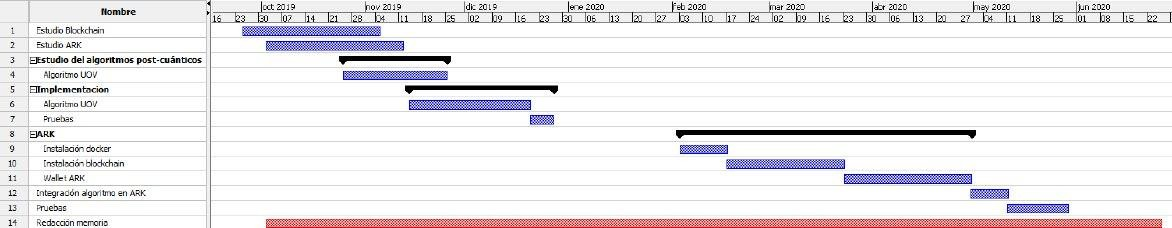
\includegraphics[width=15cm,height=5cm]{figuras/Gantt_ini.jpg}
	\caption{Comparativa de la capacidad de cómputo de un ordenador clásico con un ordenador cuántico\cite{clasica-vs-cuantica}}
	\label{fig:comp-clasica-cuantica}
\end{figure}